\chapter{Dise\~no de la soluci\'on}

% **************************** Define Graphics Path **************************
\ifpdf
    \graphicspath{{Chapter3/Figs/Raster/}{Chapter3/Figs/PDF/}{Chapter3/Figs/}}
\else
    \graphicspath{{Chapter3/Figs/Vector/}{Chapter3/Figs/}}
\fi

Durante el desarrollo de un proyecto de esta naturaleza, se plantean interrogantes, problemas, soluciones a estas interrogantes y problemas, y se toman decisiones. Estas decisiones pueden ser de diferente \'indole. 

En este capitulo nos interesamos por aquellos problemas e interrogantes y principalmente aquellas decisiones, que impactan en el dise\~no del prototipo.\\

Por otro lado, SDN es una abstracci\'on, un enfoque a seguir. Por ello, dise\~nar una soluci\'on tecnol\'ogica basada en este enfoque implica una gran cantidad de decisiones de dise\~no en particular. Algunas de ellas son que arquitectura basada en SDN utilizar, que propuesta utilizar para el software de control, como se construye un dispositivo compatible con el plano de control de SDN y en particular partiendo del hardware NetFPGA, entre otras decisiones. En el presente cap\'itulo se intenta brindar una respuesta a todas estas interrogantes, comenzando por la elecci\'on de la arquitectura SDN a utilizar. Luego se presenta el dise\~no asumido para la construcci\'on del router opensource, y sus principales componentes. Tambi\'en se presentan las componentes que constituyen a la entidad Controlador dentro del prototipo, y finalmente se detalla el dise\~no de la aplicaci\'on encargada de implementar el plano de control SDN.
 
\section[Elecci\'on de una arquitectura SDN]{Elecci\'on de una arquitectura SDN}

%En el cap\'itulo dedicado al estado del arte de las redes definidas por software, se explica en profundidad la arquitectura de SDN, y a partir del mismo queda completamente sanjada la diferencia entre los conceptos de SDN y OpenFlow por ejemplo.\\

%Entonces, la primer decisi\'on de dise\~no importante a tener en cuenta es por cual implementaci\'on del enfoque SDN optar, puesto que las alternativas existentes son bien diferentes.\\
 
Naturalmente, la primer decisi\'on de dise\~no importante a tomar, es la elecci\'on de una de las arquitecturas existentes basadas en el enfoque SDN.\\
  
Dentro de las alternativas existentes, OpenFlow se presenta como una opci\'on madura y probada[poner referencia a oefelia, google no se que y algo mas]. Como se menciono en el estado del arte OpenFlow  se ha caracterizado por un desarrollo sostenido y una amplia adopci\'on tanto por la academia como por la industria; adem\'as de ser compatible con una amplia variedad de tecnolog\'ias. Debido a esto cuenta con una amplia comunidad de usuarios, extensa documentaci\'on y es soportado por varias soluciones comerciales[referencia a switch hp, carajo carjao]. Finalmente se puede agregar que OpenFlow esta integramente desarrollado bajo la filosof\'ia opensource. Por estas razones, se decide por OpenFlow como la implementaci\'on del enfoque SDN a utilizar.\\

%[METER EN EL ESTADO DEL ARTE PARA JUSTIFICAR]
%nace como idea en el a\~no 2008, y luego de varias versiones de desarrollo libera su primera versi\'on oficial(OpenFlow v1.0.0) a finales del a\~no 2009. Tras ello se ha caracterizado por un desarrollo sostenido, siendo actualmente su versi\'on oficial la 1.5.
%[FIN]




%Por otro lado en las sucesivas versiones de OpenFlow, se han incorporado diferentes caracter\'isticas y funcionalidades que hacen en la actualidad a la versi\'on 1.5 de OpenFlow, una alternativa vers\'atil, flexible y completa.\\

Tomada la decisi\'on de utilizar OpenFlow, resta decidir en relaci\'on a esto que versi\'on utilizar.\\
Al momento de culminar el desarrollo de este trabajo, la versi\'on m\'as reciente de OpenFlow era la 1.5, mientras que al momento de iniciarse este proyecto la versi\'on m\'as reciente era la 1.4.\\

Por otro lado, la versi\'on de OpenFlow elegida debe garantizar ciertos requerimientos de diseni\~no a los que el prototipo esta sujeto. En particular interesa que garantice:

\begin{itemize}
\item Soporte para MPLS, tanto en la capacidad de reconocer los cabezales MPLS como para la manipulaci\'on de los mismos mediante las primitivas POP, PUSH y SWAP
\item Soporte para tags de VLAN (esta ultima no se si ponerla)
\end{itemize}

Sobre la primer restricci\'on, OpenFlow brinda soporte completo para MPLS a partir de la versi\'on 1.3. Por otro lado en relaci\'on a la segunda restricci\'on [COMPLETAR].\\

De esta forma, la versi\'on m\'as b\'asica de OpenFlow que asegura soporte a las restricciones de dise\~no mencionadas es la versi\'on 1.3.\\

M\'as adelante veremos en la siguiente secci\'on, la cual  esta destinada a la programaci\'on de la placa NetFPGA, que es de inter\'es trabajar con la versi\'on de OpenFlow m\'as sencilla y minimalista posible, que de soprte a todas las funcionalidades y restricciones impuestas sobre el protot\'ipo.\\ 

En conclusi\'on la versi\'on de OpenFlow a utilizar es la 1.3.

\section[Alternativas de dise\~no para el router]{Alternativas de dise\~no para el router}

Como se mencion\'o anteriormente, una de las premisas para la elaboraci\'on del router opensource es la utilizaci\'on del hardware NetFPGA. A su vez, partiendo de este hardware es necesario llegar a un dispositivo compatible con OpenFlow.\\ 

Existen dos estrategias bien definidas para la construcci\'on un switch OpenFlow, partiendo del hardware mencionado, y utilizando los diferentes proyectos disponibles para la programaci\'on del mismo. Una de ellas es programar el hardware para que se comporte como un switch compatible con el protocolo OpenFlow. La otra alternativa es programar el hardware para que se comporte como una tarjeta de red estandar, e implementar todo el comportamiento de un switch OpenFlow en software.\\

Para la primer estrat\'egia se cuenta con un proyecto desarrollado previamente para la plataforma NetFPGA, y disponible libremente en el repositorio de software de dicho producto. No obstante este proyecto presenta una dificultad y es que a pesar de haber sido dise\~ado para soportar en un futuro cualquier versi\'on disponible del protocolo OpenFlow, en su veri\'on actual solamente soporta un conjunto reducido de funcionalidades de la versi\'on 1.0 de este protocolo. \\
Como se mencion\'o anteriormente la versi\'on m\'as b\'asica de este protocolo que permite soportar el conjunto de funcionalidades relevadas como requerimientos para este proyecto es la versi\'on 1.3. Esto conlleva a la ncesidad de extender el proyecto existente, para soprtar las nuevas caracter\'isticas incorporadas en las sucesivas versiones posteriores a la 1.0; o al menos aquellas que son escenciales para soportar las caracter\'isticas pretendidas sobre el prototipo.\\

Para la segunda estrat\'egia se cuenta con un proyecto tambi\'en desarrollado previamente para la plataforma NetFPGA, llamado ReferenceNIC. Este proyecto habilita a programar el hardware para que se comporte como una placa de red estandar. Adicionalmente se debe incluir o desarrollar herramientas que permitan implementar por software el comportamiento de un switch OpenFlow. En particular sobre este \'ultimo punto vale la pena destacar la existencia de Open vSwitch, herramienta que entre otras caracter\'isticas realiza esto mismo, utilizando hardware tradicional como una placa de red estandar.

Contextualizando ambas alternativas en el marco de la realizaci\'on de este proyecto de fin de carrera, ambas alternativas presentan sus ventajas y desventajas; no siendo ninguna de ellas a priori mejor que la otra. Por ello a continuaci\'on se exponen comparativamente las principales ventajas y desventajas de cada alternativa, a modo de sustentar la elecci\'on de una ellas. 

\newpage
%%% Tabla Ventajas y Desventajas de ambas alternativas
\begin{table}[!Ht]\centering\small
\begin{tabularx}{\textwidth}{|>{\setlength\hsize{1.0\hsize}\setlength\linewidth{\hsize}}X|>{\setlength\hsize{1.0\hsize}\setlength\linewidth{\hsize}}X|}
\hline
\multicolumn{2}{|c|}{Ventajas}\\ \hline 
\hline
Extender proyecto OpenFlow NetFPGA & ReferenceNIC + Open vSwitch\\
\hline
\begin{itemize}
\item \'Optimo aprovechamiento de la capacidad de c\'omputo y procesamiento del hardware disponible.
\item Mayor posibilidad de lograr velocidades de procesamiento competitivas con productos comerciales similares.
\item Mayor posibilidad de obtener resultados aceptables, en performance y rendimiento para puesta en producción.

\end{itemize}
&
\begin{itemize}
\item No se tiene la necesidad de modificar o desarrollar software en el lenguaje y en el entorno de programaci\'on de la tarjeta NetFPGA.

\item Evitar desarrollar software para la NetFPGA ahorra tiempo de proyecto que se puede invertir en otras l\'ineas de trabajo, igualmente importantes. 

\item Programar el harware NetFPGA con proyectos precompilados como el ReferenceNIC requiere \'unicamente de licencias de software que son accesibles sin costo ya sea mediante licencias gratuitas o de prueba.
\end{itemize}
\\
\hline
\end{tabularx}
\end{table}

\begin{table}[!HT]\centering\small
\begin{tabularx}{\textwidth}{|>{\setlength\hsize{1.0\hsize}\setlength\linewidth{\hsize}}X|>{\setlength\hsize{1.0\hsize}\setlength\linewidth{\hsize}}X|}
\hline
\multicolumn{2}{|c|}{Desventajas}\\ \hline
\hline
Extender proyecto OpenFlow NetFPGA & ReferenceNIC + Open vSwitch\\
\hline
\begin{itemize}

\item Extender el proyecto existente, en si mismo constituye un empresa del porte de un proyecto de fin de carrera
\item El conocimiento técnico necesario se perfila m\'as al de un Ingeniero Eléctrico que al de un Ingeniero en Computación, lo cual constituye un riesgo del proyecto.
\item Desarrollar software para el hardware NetFPGA y compilarlo requiere de licencias de software costosas.
\end{itemize}

&

\begin{itemize}
\item No se aprovecha de forma óptima las capacidades de procesamiento del hardware disponible. En otras palabras se tiene hardwre ``caro'' y potente en forma ociosa.
\item Los resultados obtenidos en relaci\'on al rendimiento del prototipo, muy probablemente no sean los esperados para una equipo de producción.
\end{itemize}
\\
\hline
\end{tabularx}
\end{table}

\clearpage
\newpage
Habiendo presentado las principales ventajas y desventajas de cada alternativa, y teniendo presente el alcance y el tiempo disponible para la ejecuci\'on de este proyecto, se opt\'o por la segunda estrat\'egia presentada.\\

Optando por la segunda estrat\'egia presentada se logra obtener de forma temprana un prototipo de switch OpenFlow con el cual trabajar en la programaci\'on del datapath mediante un controlador, desarrollar estrategias para constru\'ir servicios en una red h\'ibrida IP/MPLS, as\'i como dise\~nar pruebas y un testbed acorde para validar tecnol\'ogicamente la soluci\'on propuesta.\\ 


\section[Alternativas de dise\~nio]{Plano de Control centralizado vs distribu\'ido}

\section[Dise\~no general del prototipo]{Dise\~no general del prototipo}

En esta secci\'on se presenta a modo de resumen de las secciones anteriores, la estructura general que adopta la soluci\'on, al asumir las decisiones de dise\~no discutidas anteriormente.\\

Comenzando con la estructura del router, en ~\ref{fig:OpenSourceRArch} puede apreciarse las principales componentes que lo constituyen; tanto a nivel de hardware como de software.\\
Enfocandos\'e en las componentes del hardware, el router se compone de una PC de escritorio convencional y una tarjeta NetFPGA, programada con el proyecto Reference NIC. Por detalles en particular respecto de la arquitectura de dicha PC refierase al anexo [link al anexo].\\  
Por otro lado en relaci\'on a las componentes de software, el router se compone de un sistema operativo escritorio basado en linux, con las instalaciones de Open vSwitch, Quagga y el agente de gesti\'on SNMP. Nuevamente por mayores detalles acerca de las versiones de software utilizadas, sistema operativo entre otros detalles refierase al anexo [link al anexo].\\

\newpage
\begin{figure}[htbp!] 
\centering    
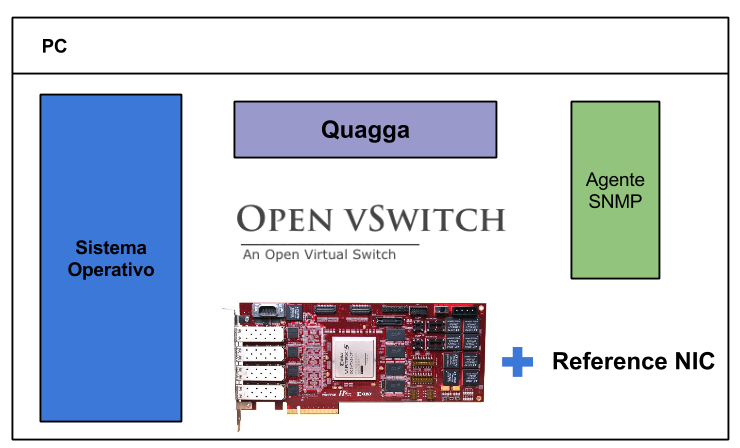
\includegraphics[width=0.7\textwidth]{Arch_Figure1}
\caption[OpenSourceRArch]{Diagrama de componentes del router open source}
\label{fig:OpenSourceRArch}
\end{figure}

Luego como puede verse en la imagen ~\ref{fig:OpenSourceRArch2}, el router es programado por la entidad Controlador, mediante el protocolo de comunicaci\'on OpenFlow.


\begin{figure}[htbp!] 
\centering    
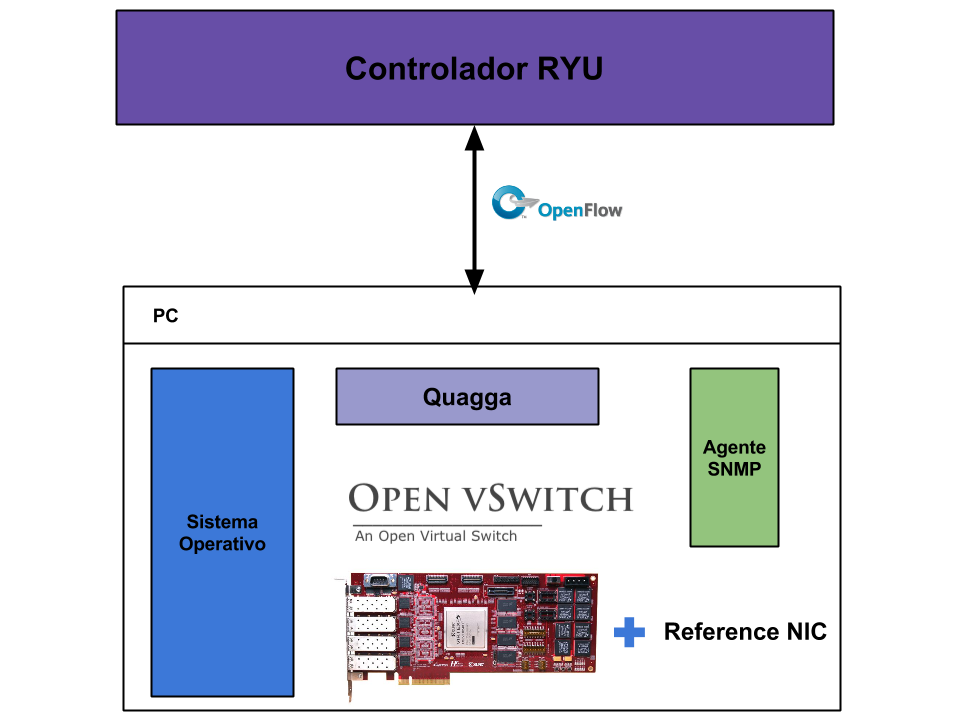
\includegraphics[width=0.7\textwidth]{Arch_Figure2}
\caption[OpenSourceRArch2]{Interacci\'on entre Router y Controlador}
\label{fig:OpenSourceRArch2}
\end{figure}

\newpage
Con respecto al Controlador, vale la pena destacar solamente las componentes de software dado que en relaci\'on al hardware, el mismo esta basado en una PC de escritorio. En la imagen ~\ref{fig:OpenSourceRArch3} se aprecian los componentes que constituyen al Controlador.\\

Al igual que el router, el Controlador consta de un sistema operativo sobre el cual posteriormente se instalan las diferentes componentes de software utilizadas. Particularmente esta compuesto por la suite de ruteo Quagga, un modulo encargado de la sincronizaci\'on de la informaci\'on topl\'ogica, un gerente SNMP, y finalmente el software de control SDN Ryu, sobre el cual se ejecuta la aplicaci\'on RauFlow.

\begin{figure}[htbp!] 
\centering    
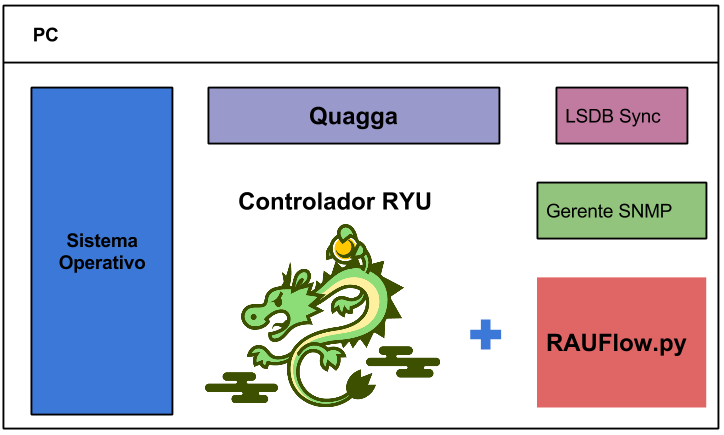
\includegraphics[width=0.6\textwidth]{Arch_Figure3}
\caption[OpenSourceRArch3]{Diagrama de componentes del Controlador}
\label{fig:OpenSourceRArch3}
\end{figure}

De esta forma, el prototipo para la nueva versi\'on de la red acad\'emica, se compone principalmente de algunos nodos construidos en base al router open source, y un dispositivo controlador. Como se puede observar en la imagen \ref{fig:OpenSourceRArch4} los nodos se comunican con el Controlador mediante el protocolo OpenFlow como se explico con anterioridad, habilitando de esta forma a que el plano de datos sea programado por el plano de control. Por otro lado las diferentes instancias de Quagga distribu\'idas en cada nodo de la red y en el dispositivo controlador, se comunican mediante un canal IP con el objetivo de aprender la topolog\'ia y diseminar la informaci\'on de ruteo. Finalmente el gerente SNMP interactua con los diferentes agentes SNMP localizados en cada nodo mediante el canal IP, para obtener infirmaci\'on adicional acerca de cada nodo. 

\begin{figure}[htbp!] 
\centering    
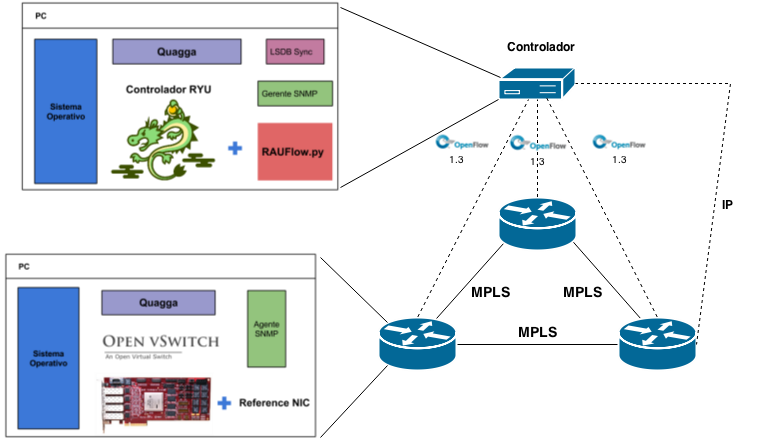
\includegraphics[width=0.9\textwidth]{Arch_Figure4}
\caption[OpenSourceRArch4]{Vista l\'ogica del prototipo}
\label{fig:OpenSourceRArch4}
\end{figure}

\newpage
\section[RAUFlow]{RAUFlow}

En las secciones anteriores se ha explicado en detalle las caracter\'isticas m\'as importantes del prototipo, as\'i como las principales componentes del router open source y del dispositivo controlador. 
Resta detallar entonces, el dise\~no de la aplicaci\'on que correr\'a en el dispositivo controlador y ser\'a encargada de implementar el plano de control; de aqu\'i en m\'as RauFlow. Por ello en la siguiente secci\'on se propone un an\'alisis de dicha componente, siguiendo un proceso de dise\~no tradicional de Ingenier\'ia de Software, dividido en 4 etapas. Una primera etapa de an\'alisis de requerimientos, una segunda etapa de relevamiento de casos de uso, una tercera etapa de dise\~no del modelo de datos, y finalmente una cuarta etapa para el dise\~no general de la arquitectura de la aplicaci\'on.  

\subsection[An\'alisi de requerimientos]{An\'alisis de requerimientos}

Anteriormente se han descrito los requerimientos relevados para el prototipo definido en este trabajo. De ellos y de un trabajo de an\'alisis sobre la realidad modelada, se desprende la siguiente tabla de requerimientos.

\clearpage
\begin{table}[Htl]\centering
\begin{tabularx}{\textwidth}{|>{\setlength\hsize{1.0\hsize}\setlength\linewidth{\hsize}}X|}
\hline
Requerimientos Funcionales\\ \hline
\hline
\begin{itemize}
\item El Sistema debe de proveer la facilidad para obtener la informaci\'on asociada a cada nodo de la red, permitiendo a su vez agregar informaci\'on que facilite la identificaci\'on del mismo para un usuario.
\item El Sistema debe proveer la facilidad para agregar, modificar y eliminar redes virtuales. 
%En particular al trabajar con redes virtuales y sus datos, se debe soportar el manejo de datos como la numeraci\'on IP del tr\'afico asociado a una red virtual, informaci\'on de capa de transporte, entre otros.
\item El Sistema debe proveer la facilidad para obtener toda la informaci\'on relevante de una red virtual.
\item El Sistema debe permitir visualizar de alguna forma los caminos constru\'idos para encaminar el tr\'afico de una red virtual en particular, a trav\'es de la red del protot\'ipo.
\item El Sistema debe proveer la facilidad para visualizar el estado de las tablas de flujos asociadas a cualquier nodo de la red del protot\'ipo.
\end{itemize}\\
\hline
\end{tabularx}
\end{table}

\begin{table}[Htl]\centering
\begin{tabularx}{\textwidth}{|>{\setlength\hsize{1.0\hsize}\setlength\linewidth{\hsize}}X|}
\hline
Requerimientos no Funcionales\\ \hline
\hline
\begin{itemize}
\item Se debe utilizar siempre que sea posible herramientas de software libre y c\'odigo abierto.
\end{itemize}\\
\hline
\end{tabularx}
\end{table}

Teniendo en cuenta la descripci\'on del problema y los requerimientos anteriores, se procedio con el modelado de la realidad. Los resultados obtenidos se presentan en la siguiente secci\'on.

%Teniendo en cuenta los requerimientos anteriores, se procede con el relevamiento de los casos de uso. Los resultados obtenidos se presentan en la siguiente secci\'on.

\subsection[Modelado de la realidad]{Modelado de la realidad}

En la figura ~\ref{fig:ModeloDeDominio} se presenta el modelo de dominio realizado a partir de la realidad a modelar. En el mismo se destacan en color amarillo aquellas entidades que se entiende se corresponden al modelado de la topolog\'ia y sus diferentes elementos como lo son los Nodos y sus Interfaces. Por otro lado en rosado se destacan aquellas entidades relacionadas al concepto de MPLS, que se consideran importantes; como lo son las tablas FTN, ILM y NHLFE. Finalmente vale la pena destacar el concepto de Servicio, con el cual se decidi\'o representar a las redes virtuales soportadas en el protot\'ipo. Interesa destacar adem\'as del concepto de Servicio, que es una redefinici\'on desde una visi\'on centralizada del concepto FEC en la teor\'ia de MPLS, concepto que en la literatura de MPLS tradicional esta vinculado a un solo nodo en una red, y no a muchos como se propone en este trabajo.  

\begin{figure}[ht!] 
\centering    
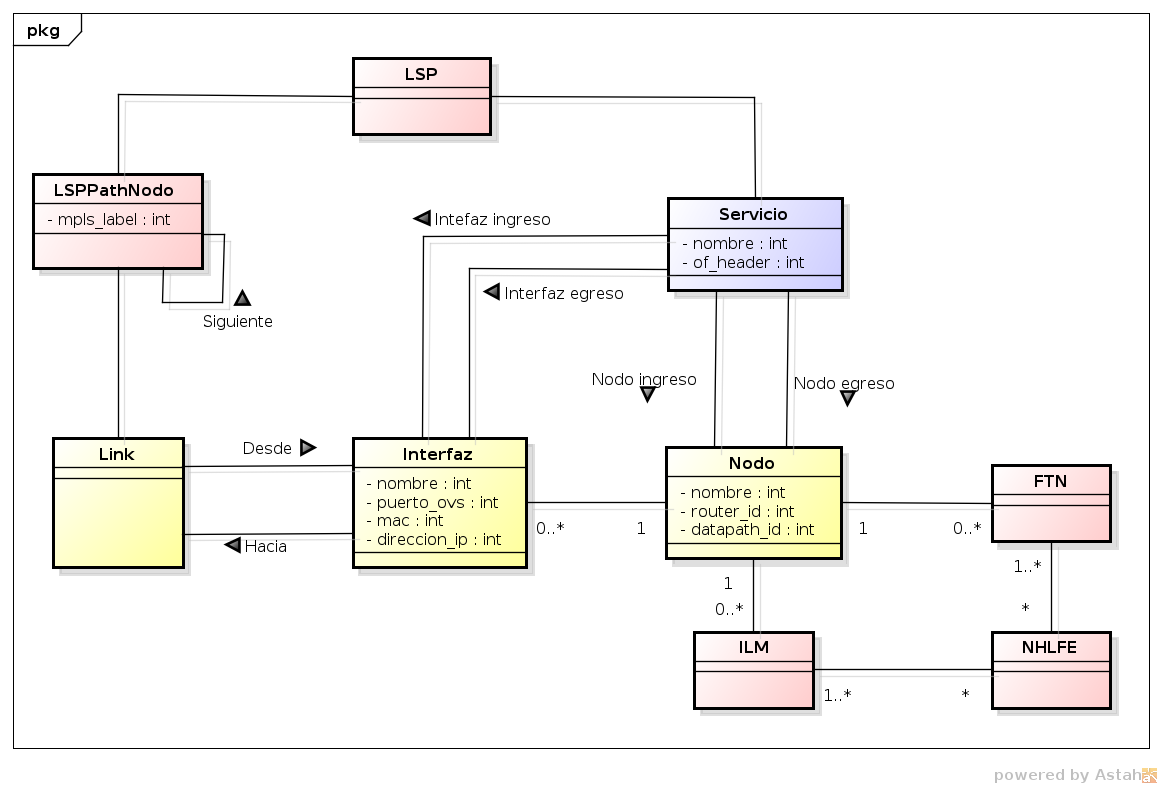
\includegraphics[width=0.7\textwidth]{Disenio_Figure1}
\caption[ModeloDeDominio]{Modelo de Dominio}
\label{fig:ModeloDeDominio}
\end{figure}

Sobre este modelo de dominio se trabaj\'o hasta llegar finalmente al diagrama de clase de dise\~no que se presenta a continuaci\'on en la figura [ref].\\

Teniendo en cuenta los requerimientos mencionados, y el modelado de la realidad presentado, se procede con el relevamiento de los casos de uso. Los resultados obtenidos se presentan en la siguiente secci\'on.

\subsection[Relevamiento de casos de uso]{Relevamiento de casos de uso}

La lista de casos de uso presentada a continuaci\'on se corresponde con un conjunto de funcionalidades b\'asicas, que permitan la exploraci\'on de la potencialidad del enfoque SDN aplicado a nuestro problema. 

\begin{itemize}
\item Listar Servicios
\item Agregar Servicio
\item Modificar Servicio
\item Eliminar Servicio
\item Ver Topolog\'ia
\item Ver informaci\'on b\'asica Nodo
\item Ver tabla de Flujos Nodo
\item Filtrar Lsps
\item Editar Informaci\'on extra Nodo
\item Editar Informaci\'on extra Interfaz
\end{itemize}

De esta forma quedan presentados los requerimientos relevados sobre RauFlow, el modelado de la realidad, y los casos de uso relevados. Resta entonces presentar un esbozo de la arquitectura de la aplicaci\'on RauFlow, para que el lector finalmente este en condiciones de comprender el dise\~'no del prototipo en su totoalidad.

\subsection[Arquitectura de RauFlow]{Arquitectura de RauFlow}

En la figura ~\ref{fig:VistaComponentes2} se presenta un esquema con las componentes l\'ogicas que forman parte de la aplicaci\'on denominada RauFlow. Como se explico anteriormente, Ryu habilita la programaci\'on del plano de control mediante aplicaci\'ones desarrolladas en lenguaje Phyton con una cierta estructura particular. Por consiguiente RauFlow esta basado en al menos una aplicaci\'on de este tipo.\\

Por otro lado si bien Ryu ofrece un entorno para la ejecuci\'on de m\'ultiples aplicaciones, asi como un mecanismo para la comunicaci\'on entre ellas, por simplicidad se opto por basar el dise\~no de RauFlow en una \'unica aplicaci\'on Ryu lo m\'as simple posible. Luego funcionalidades y responsabilidades que no son previstas en dicha aplicaci\'on son implementadas por componentes adicionales, siguiendo un dise\~no modular.\\

Cabe destacar adem\'as, la existencia en el dise\~no de un conjunto de aplicaciones Ryu, dise\~nadas e implementadas por tereceros. Estas aplicaciones en particualr se encuentran dentro del conjunto de aplicaciones que vienen con el Controlador. M\'as adelante se explicar\'a en detalle cual es el rol que cumplen estas aplicaciones en el dise\~no de RauFlow.\\

En su dise\~no, RauFlow puede ser estudiado a trav\'es de 3 capas l\'ogicas. Comenzando por ejemplo por el estudio de una capa de Presentaci\'on y una capa Negocios, y terminando con el estudio de una capa de Aplicaciones Ryu.\\ 

%Esta \'ultima capa tiene sentido como tal, cuando el prototipo requiere de la ejecuci\'on de m\'ultiples aplicaciones Ryu, aspecto que ser\'a retomado m\'as adelante en esta secci\'on.\\

Empezando por el final, en la capa de Aplicaciones Ryu se encuentra el programa encargado de implementar los procesos y protocolos del plano de control. Naturalmente el mismo esta dise\~nado bajo el esquema de una aplicaci\'on Ryu. No obstante toda l\'ogica de negocios asociada a la realidad modelada se encuentra en la capa de Negocios, desacoplada totalmente de dicha aplicaci\'on. Esto obedece a un criterio de dise\~no en el cual se busca mantener la l\'ogica de la aplicaci\'on de Ryu lo m\'as simple posible, haciendola responzable \'unicamente por los eventos asociados al protocolo OpenFlow principalmente.\\ 

\begin{figure}[ht!] 
\centering    
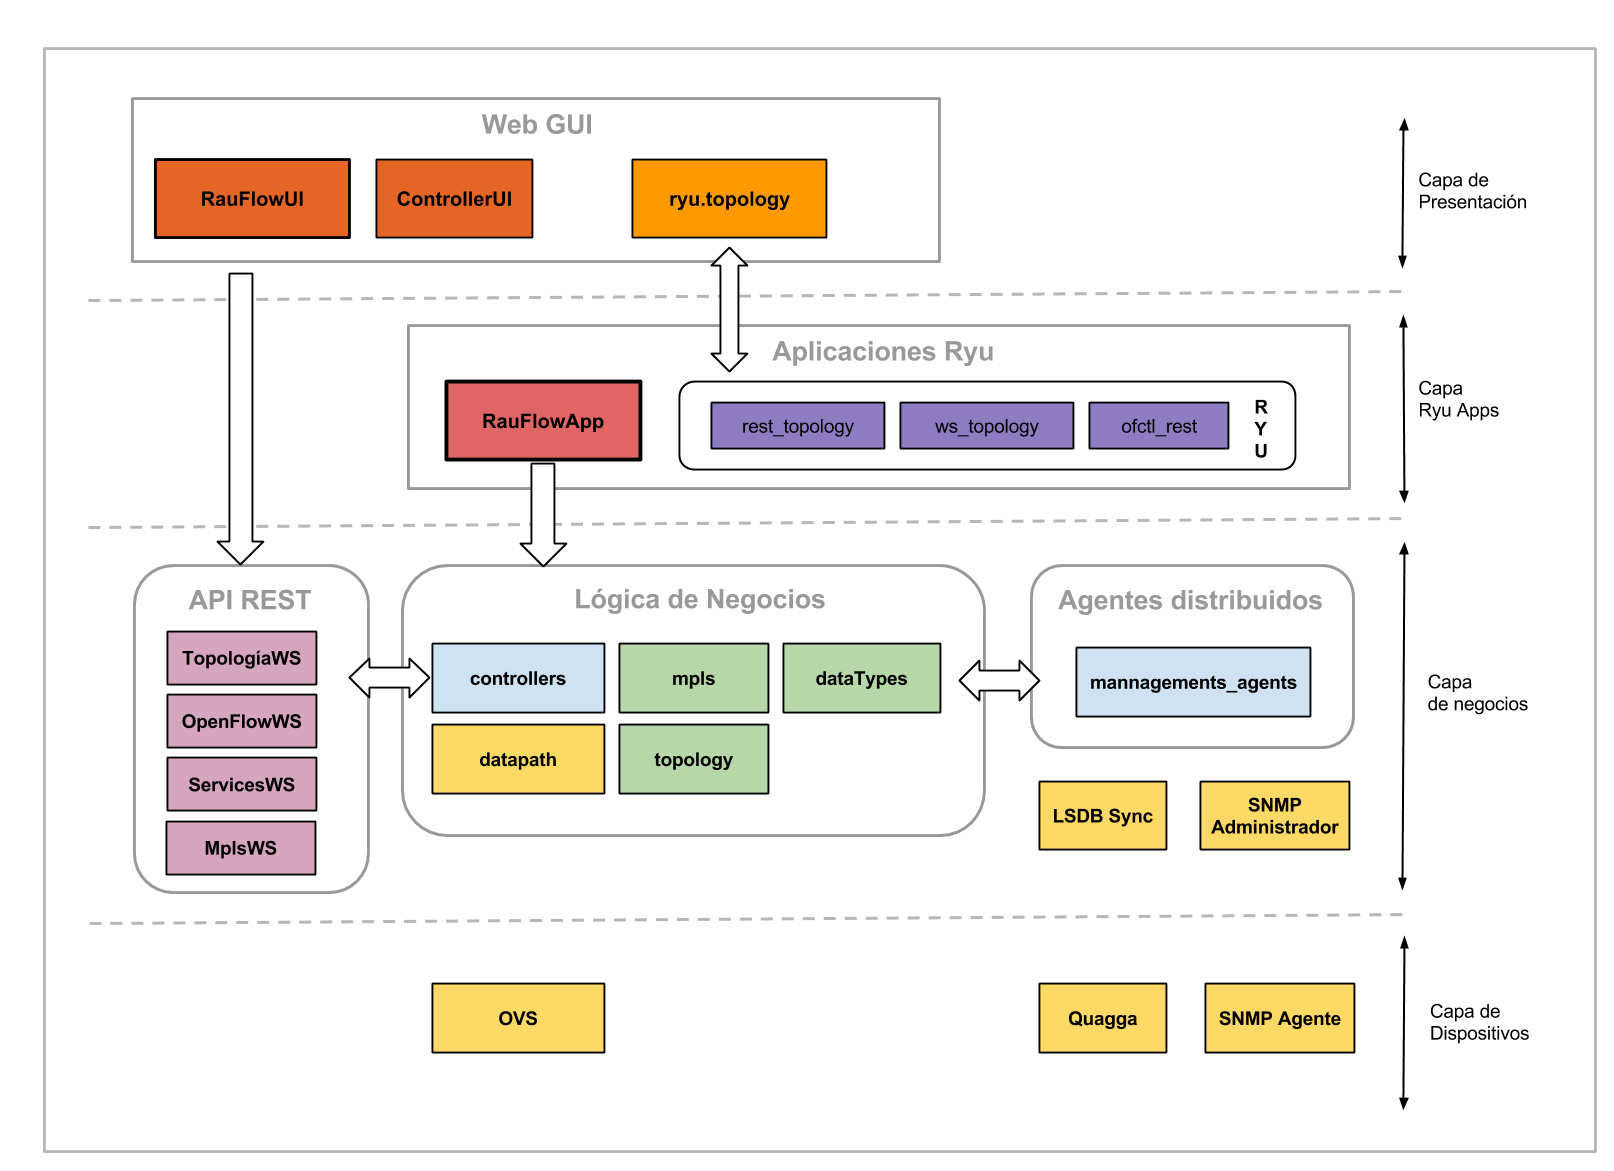
\includegraphics[width=1.0\textwidth]{Disenio_Figure3}
\caption[Vista l\'ogica]{Vista l\'ogica}
\label{fig:VistaComponentes2}
\end{figure}

Luego, en la capa de negocios se encuentran 3 componentes. Una componente de l\'ogica de negocios, puramente relacionada a la realidad modelada, una API REST de servicios para el acceso y la manipulaci\'on de datos relacionados a la primera componente, y finalmente una tercera componente denominada Agentes distribu\'idos.\\

Profundizando en la componente de l\'ogica de negocios, esta se encuentra a su vez sub-dividida en diferentes m\'odulos que agrupan funcionalidades acorde a su naturaleza y responsabilidades. De estos m\'odulos vale la pena destacar el m\'odulo \textbf{topology}, responsable de la representaci\'on de la topolog\'ia y las operaciones para la manipulaci\'on de la misma, el m\'odulo \textbf{mpls}, responsable por las operaciones y conceptos relacionados al protocolo mpls, y el modulo \textbf{datapath}, responsable del acceso y manipulaci\'on de los diferentes dispositivos del datapath propiamente dicho.\\ 

Por otro lado, enfocandose en la componente de Servicios REST, la misma se encuentra sub dividida en varios m\'odulos, respondiendo al criterio utilizado para el dise\~no modular de la componente de l\'ogica de negocios. Dicha componente comprende desde un modulo de servicios para el acceso a la informaci\'on de la topolog\'ia, un modulo de servicios para el acceso a la informaci\'on relacionada a mpls, hasta un m\'odulo de servicios para el acceso a informaci\'on de naturaleza OpenFlow vinculada a los diferentes dispositivos del datapath.\\

Finalmente, en relaci\'on a la componente denominada Agentes distribu\'idos, esta se encarga de la interacci\'on con diferentes agentes y procesos instalados en cada router opensource a traves de un canal IP. Este m\'odulo de comunicaci\'on, as\'i como los diferentes agentes instalados en cada router opensource, juegan un rol irremplazable en la obtenci\'on de informaci\'on; puesto que a partir del canal de comunicaci\'on OpenFlow solamente es accesible Open vSwitch y la informaci\'on contemplada por el protocolo OpenFlow.
Dentro de esta componente, en el diagrama se muestra un modulo denominado \textbf{managements\_ agents}. Este m\'odulo opera como una interfaz de conexi\'on entre los diferentes m\'odulos de la l\'ogica de negocios, y los diferentes m\'odulos encargados de la comunicaci\'on con cada agente distribu\'ido en particular.\\ 

Por ejemplo en la figura ~\ref{fig:VistaComponentes2} se muestran el modulo \textbf{SNMP Management}, responsable de  la comunicaci\'on con un agente SNMP distribu\'ido entre los nodos del prototipo, con el fin de obtener informaci\'on extra acerca de las interfaces de red de cada router opensource.\\

De esta forma se llega a la capa de presentaci\'on. En la misma se destacan, una interfaz gr\'afica identificada en el esquema como RauFlowUI, la cual implementa cada uno de los casos de uso mencionados anteriormente en [link a la secci\'on de casos de uso], otra componente identificada como ControladorUI la cual funciona a modo de nexo entre las funcionalidades de RauFlowUI y la API Rest de Servicios; y finalmente la componente identificada como \textbf{ryu.topology}. Esta \'ultima componente forma parte del conjunto de apliaciones Ryu adicionales que se incluyen en el dise\~no de RauFlow, y tiene como principal funci\'on la de proveer una representaci\'on gr\'afica en tiempo real de la topolog\'ia existente en el prototipo.\\

Habiendose explicado en detalle cada una de las capas l\'ogicas en el dise\~no de RauFlow, se aborda a continuaci\'on las aplicaciones Ryu desarrolladas por terceros.\\

Ryu incluye tres aplicaciones dise\~n'adas para implementar una interfaz gr\'afica. Dicha interfaz consiste en un p\'agina web implementada con html, javascript y web sockets; que permite visualizar la red en su totalidad. Estos son los dispositivos del datapath con sus interfaces, y los enlaces existentes.\\
Por esta razon se incluyen en el dise\~no del proptotipo dichas aplicaciones, con el objetivo de contribu\'ir a las funcionalidades de la capa de presentaci\'on.

%que permite visualizar de forma similar a un grafo los diferentes deispositivos del datapath.

%Deacuerdo con los objetivos de este proyecto, el desarrollo de una interfaz gr\'afica no esta necesariamente inclu\'ido dentro del alcance final. De todas formas se incluye el desarrollo de la misma como un objetivo de baja prioridad puesto que agrega valor al prototipo final. Por otro lado dentro del conjunto de aplicaciones que trae el controlador Ryu, se incluyen tres aplicaciones que ejecutandose en conjunto con una aplicaci\'on web, proporcionan una interfaz gr\'afica, cuya \'unica funcionalidad es la de mostrar la topolog\'ia actual de red mediante un grafo. Adem\'as vale la pena destacar que esta implementada en base a web sockets, por lo que la vista topol\'ogica se mantiene constantemente actualizada.\\